%!TEX root = practicum1.tex
We perform two different experiments with the Chirikov map defined in \cref{eq:chirikov}. In \cref{ss:fixed} we fix the value of the non-linearity parameter and explore the influences of different values for $p_0$ and $x_0$. In \cref{ss:variable} we discuss the influence of the non-linearity parameter $K$.

\subsection[]{Fixed $K$}
\label{ss:fixed}
	We have fixed the value of $K$ to 1, essentially removing the parameter form the equation. By choosing different initial values we can generate discrete points, close curves and orbits with \cref{eq:chirikov}.
	
	\subsubsection{Discrete points}
	The Chirikov map results in discrete points if we can remove the periodicity caused by the sinus in \eqref{eq:chirikov:p}.

	\todo[inline]{$x_0 = 0$}

	\todo[inline]{$x_0 = 0.5$}


	\todo[inline]{Are the single points or curves visited in a fixed order?}
	\todo[inline]{What happens in the filled areas?}
	
	\subsubsection{Closed curves}
	\todo[inline]{Wanneer krijgen we dit?}
	\todo[inline]{Are the single points or curves visited in a fixed order?}
	\todo[inline]{What happens in the filled areas?}

	\subsubsection{Orbits}	
	\todo[inline]{Wanneer krijgen we dit?}
	\todo[inline]{Are the single points or curves visited in a fixed order?}
	\todo[inline]{What happens in the filled areas?}


	\todo[inline]{Jeej mooie plaatjes}

	%!TEX root = practicum1.tex

\begin{figure*}
	\centering
	% \x/\picname in {4/pic1.png,8/pic2.png,15/pic3.png,16/pic4.png}
	\foreach \dim/\x/\p in {0/0.500/0.500, 1/0.1576131/0.9705928, 2/0.1269868/0.9133759}
	{ 
		\begin{subfigure}[t]{0.32\textwidth}
			\includegraphics[width=\textwidth]{./img/assignment_a_\dim_dim.pdf}
			\caption{$x_0=\num{\x}$, $p_0=\num{\p}$}
			\label{fig:experiment:dimension:\dim}
		\end{subfigure}
		\begin{subfigure}[t]{0.32\textwidth}
			\includegraphics[width=\textwidth]{./img/assignment_a_\dim_dim_progression_p.pdf}
			\caption{Progression of $p$ in \subref{fig:experiment:dimension:\dim}}
			\label{fig:experiment:dimension:\dim:x}
		\end{subfigure}		
		\begin{subfigure}[t]{0.32\textwidth}
			\includegraphics[width=\textwidth]{./img/assignment_a_\dim_dim_progression_x.pdf}
			\caption{Progression of $x$ in \subref{fig:experiment:dimension:\dim}}
			\label{fig:experiment:dimension:\dim:p}
		\end{subfigure}		
	}
	\caption{Each row corresponds to on set of initial values $\left\langle x_0, p_0 \right\rangle$. The first column shows $x_n$ versus $p_n$ for $n \in \left[0,\, \num{10000} \right]$. The second and third column depict respectively the progression of $p$ and $x$.}
	\label{fig:experiment:dimension}
\end{figure*}

	\begin{figure}
		\centering
		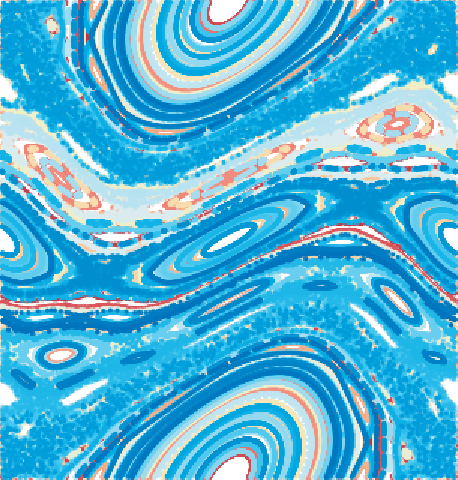
\includegraphics[width=0.9\columnwidth]{./img/assignment_a_pretty_low_res.pdf}
		\caption{500 randomly initialized orbits of the Frenkel-Kontorova model for $K = 1$.}
		\label{fig:a:pretty}
	\end{figure}

\subsection[]{Variable $K$}
\label{ss:variable}